\documentclass[fleqn]{article}
\usepackage[spanish]{babel}
\usepackage{amsmath}
\usepackage{amsthm}
\usepackage{graphicx}
\usepackage[utf8]{inputenc}

%%%%%%%% MARGIN
\usepackage[left=1in, right=1in, top=0.8in, bottom=0.8in]{geometry}

%%%%%%%% NO PARAGRAPH INDENT
% https://tex.stackexchange.com/questions/27802/set-noindent-for-entire-file
\setlength\parindent{0pt}

%%%%%%%% SUB-FIGURE PACKAGE
\usepackage{subcaption}

%%%%%%%% HYPERREF PACKAGE
\usepackage{hyperref}
\hypersetup{linkcolor=blue}
\hypersetup{citecolor=blue}
\hypersetup{urlcolor=blue}
\hypersetup{colorlinks=true}

%%%%%%%% MULTI-COLUMNS PACKAGE
\usepackage{multicol}

%%%%%%%% SETS DEFINITIONS
\usepackage{amssymb}
%%%% Important sets
\renewcommand{\O}{\mathbb{O}}
\newcommand{\N}{\mathbb{N}}
\newcommand{\Z}{{\mathbb{Z}}}
\newcommand{\Q}{{\mathbb{Q}}}
\newcommand{\R}{{\mathbb{R}}}

%%%% Statistics
\newcommand{\E}[1]{\mathbb{E}\left[#1 \right]}
\newcommand{\V}[1]{\mathrm{Var}\left[#1 \right]}

%%%% Lambda Calculus Symbols
\newcommand{\dneq}{\,\, \# \,\,}
\renewcommand{\S}{\pmb{\mathrm{S}}}
\newcommand{\I}{\pmb{\mathrm{I}}}
\newcommand{\K}{\pmb{\mathrm{K}}}
\newcommand{\ch}[1]{\ulcorner #1 \urcorner}

%%%% Ordinal Lambda Calculus Symbols
\newcommand{\ordAlph}{\Sigma_{\text{Ord}}}
\newcommand{\termOrd}{\text{Term}_\text{Ord}}
\newcommand{\fl}{\mathrm{fl}}
\newcommand{\sk}{\mathrm{sk}}

%%%% Superscript to the left
% https://latex.org/forum/viewtopic.php?t=455
\usepackage{tensor}
\newcommand{\app}[3]{\tensor*[^{#1}]{\left(#2, #3\right)}{}}

%%%% Make optional parameter
% https://tex.stackexchange.com/questions/217757/special-behavior-if-optional-argument-is-not-passed
\usepackage{xparse}
\NewDocumentCommand{\cx}{o}{
  \IfNoValueTF{#1}
  {\left[\quad\right]}
  {\left[\, #1 \,\right]}
}

%%%%%%%% LOGIC TREES
\usepackage{prftree}

%%%%%%%% SPLIT EQUATIONS
% https://tex.stackexchange.com/questions/51682/is-it-possible-to-pagebreak-aligned-equations
\allowdisplaybreaks

%%%%%%%% CODE RENDERING
% Compile with flag -shell-escape
% \usepackage{minted}

%%%%%%%% EXAM PACKAGE
\usepackage{mathexam}

%%%%%%%% CHANGE MARGINS ITEMIZE
\usepackage{enumitem}

\usepackage{float}

%%%%%%%% START DOCUMENT

\ExamClass{ANÁLISIS NUMÉRICO}
\ExamName{EXAMEN 1}
\ExamHead{\today}

\let\ds\displaystyle

\begin{document}
 \vspace{0.3cm}
   % Information of the student
   \begin{itemize}[leftmargin=6.25cm, labelsep=0.5cm]

     \item[\textit{Nombre}] \scalebox{1.2}{Juan Sebastián Cárdenas Rodríguez} % Name
     \item[\textit{Código}] 201710008101 % Code

   \end{itemize}

   \begin{enumerate}
     \item Pregunta 1.
       \begin{enumerate}
         \item Item 1.
         \begin{figure}[H]
           \centering
           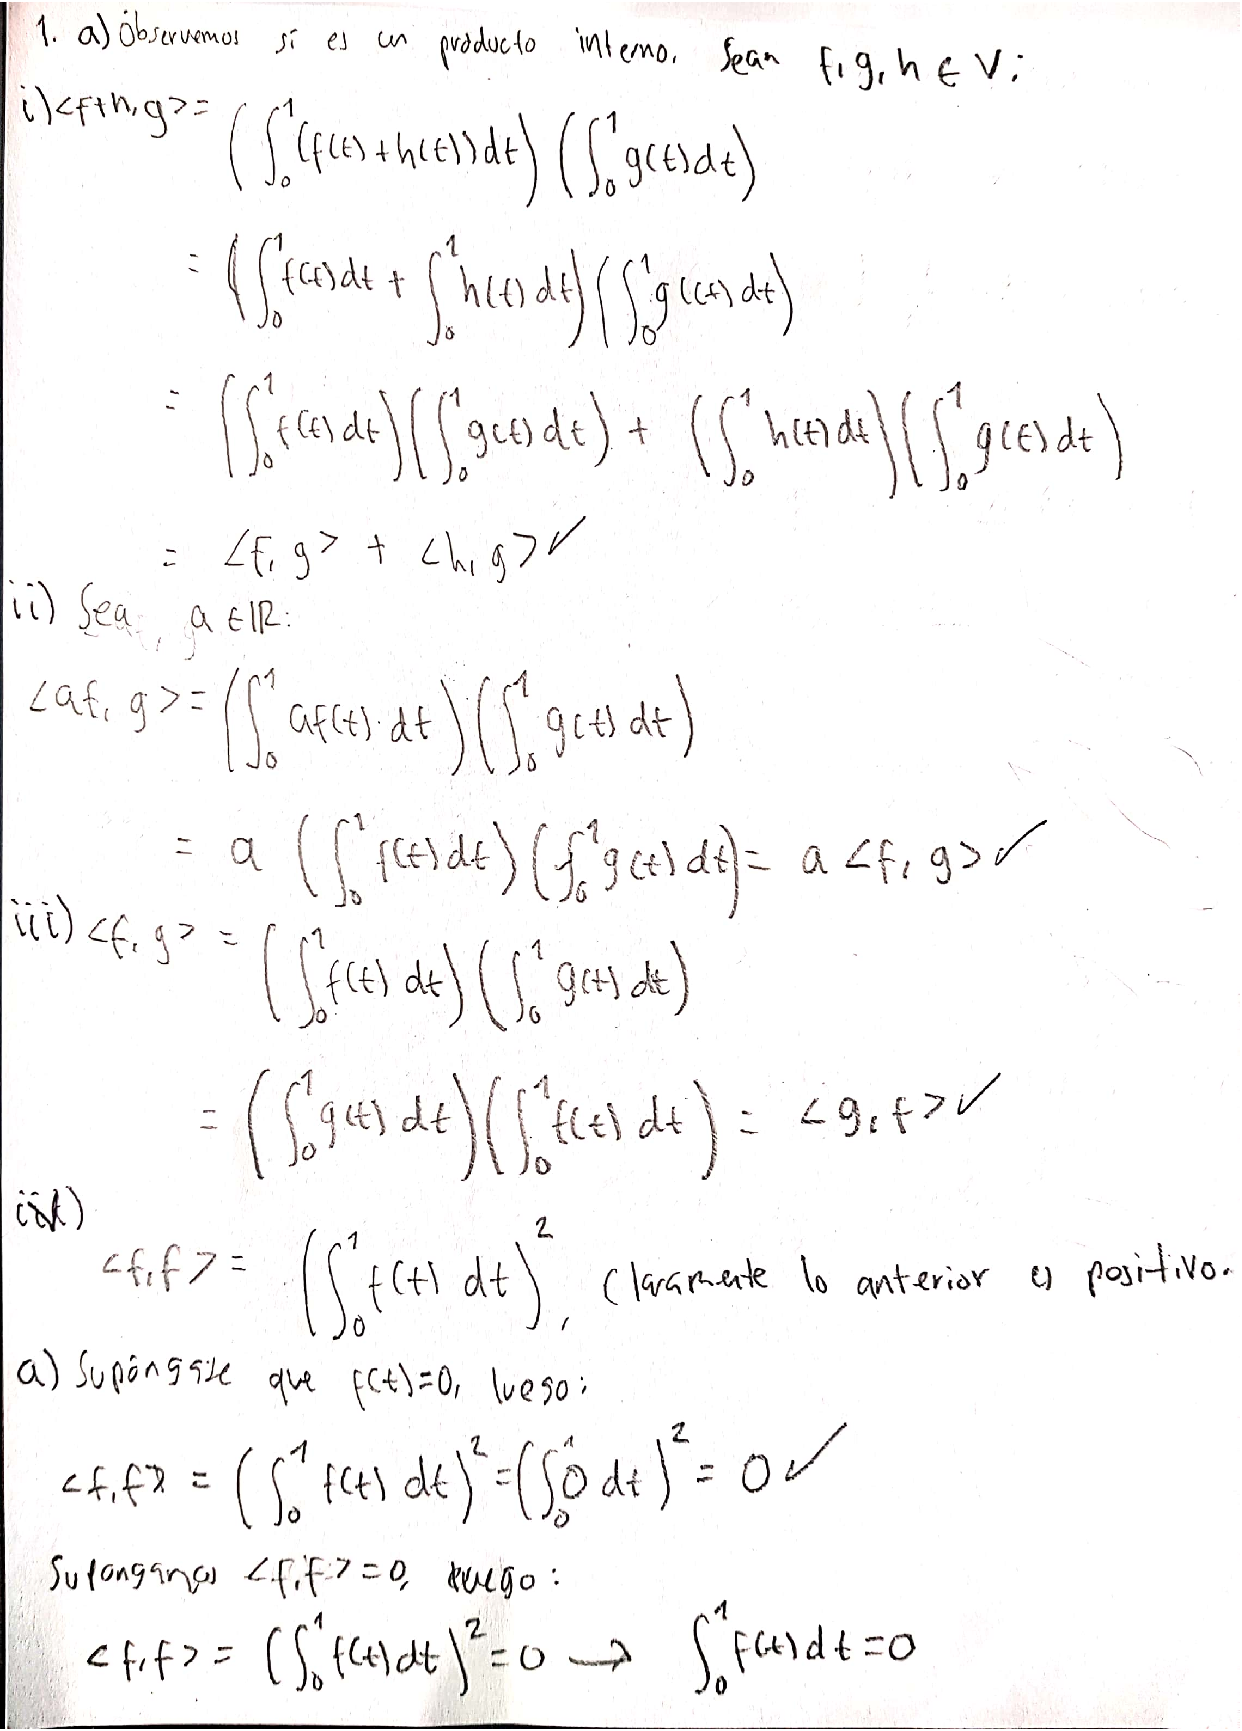
\includegraphics[scale=.6]{figs/1a1}
         \end{figure}
         \begin{figure}[H]
           \centering
           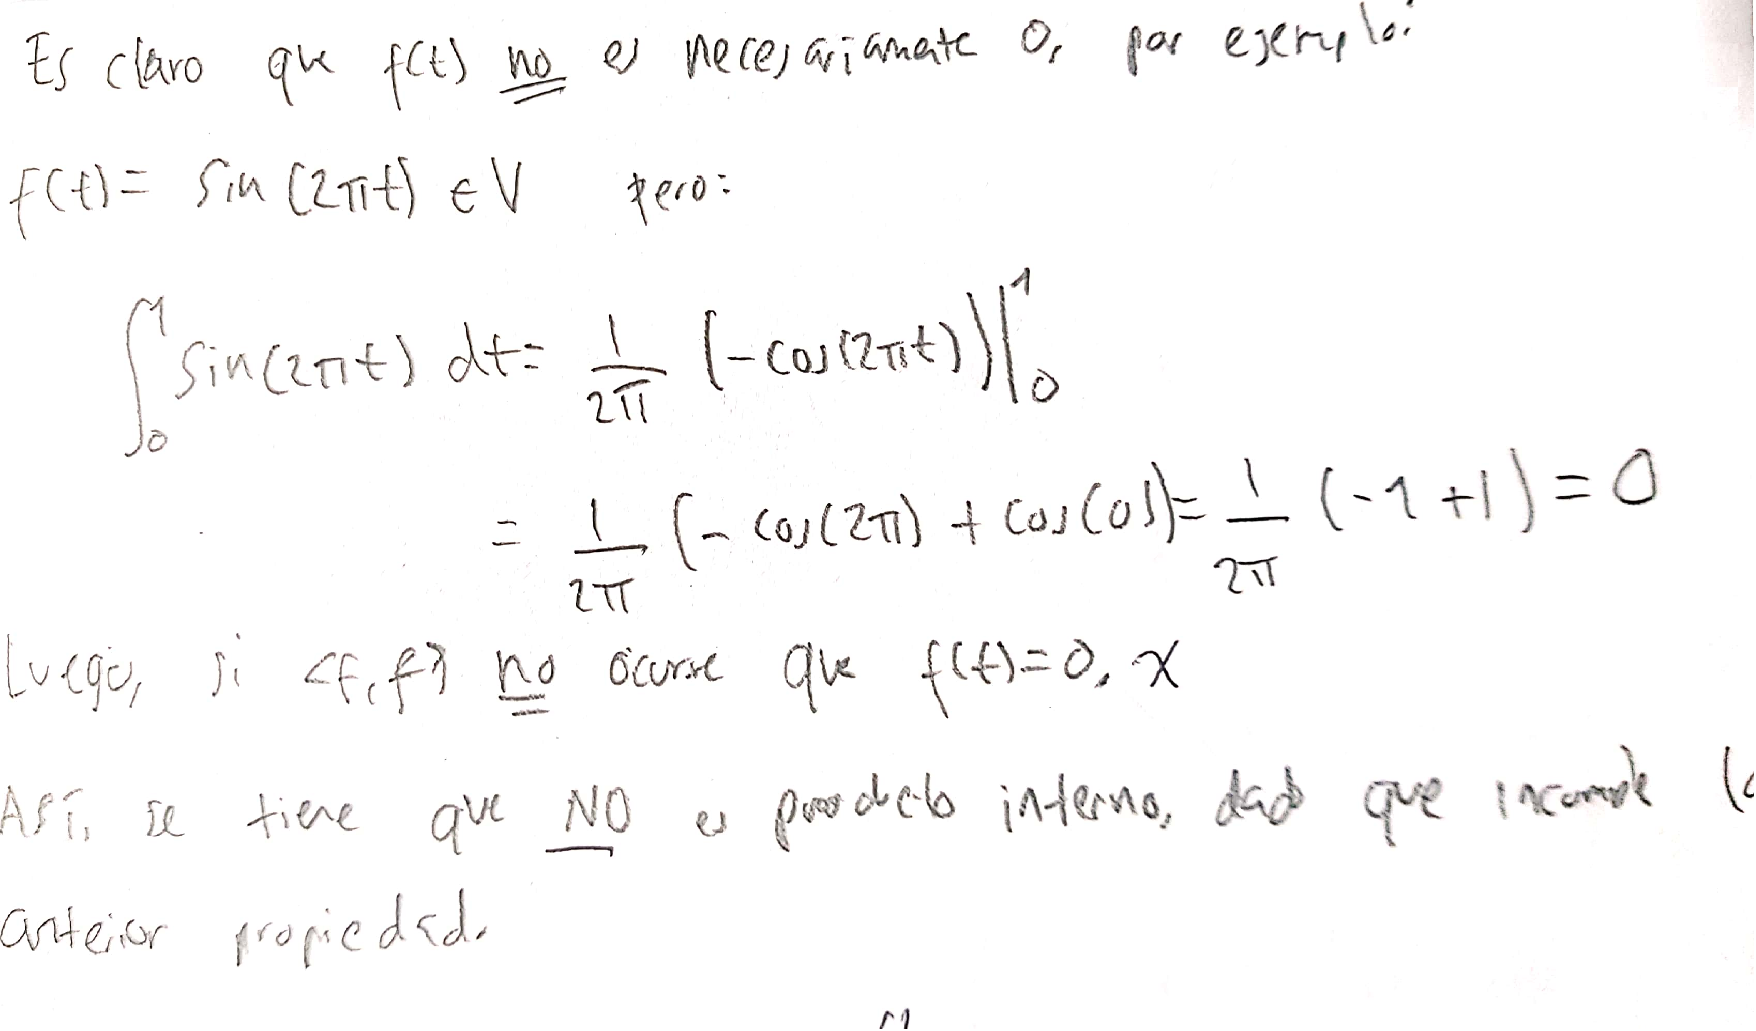
\includegraphics[scale=.5]{figs/1a2}
         \end{figure}
         \item Item 2.
         \begin{figure}[H]
           \centering
           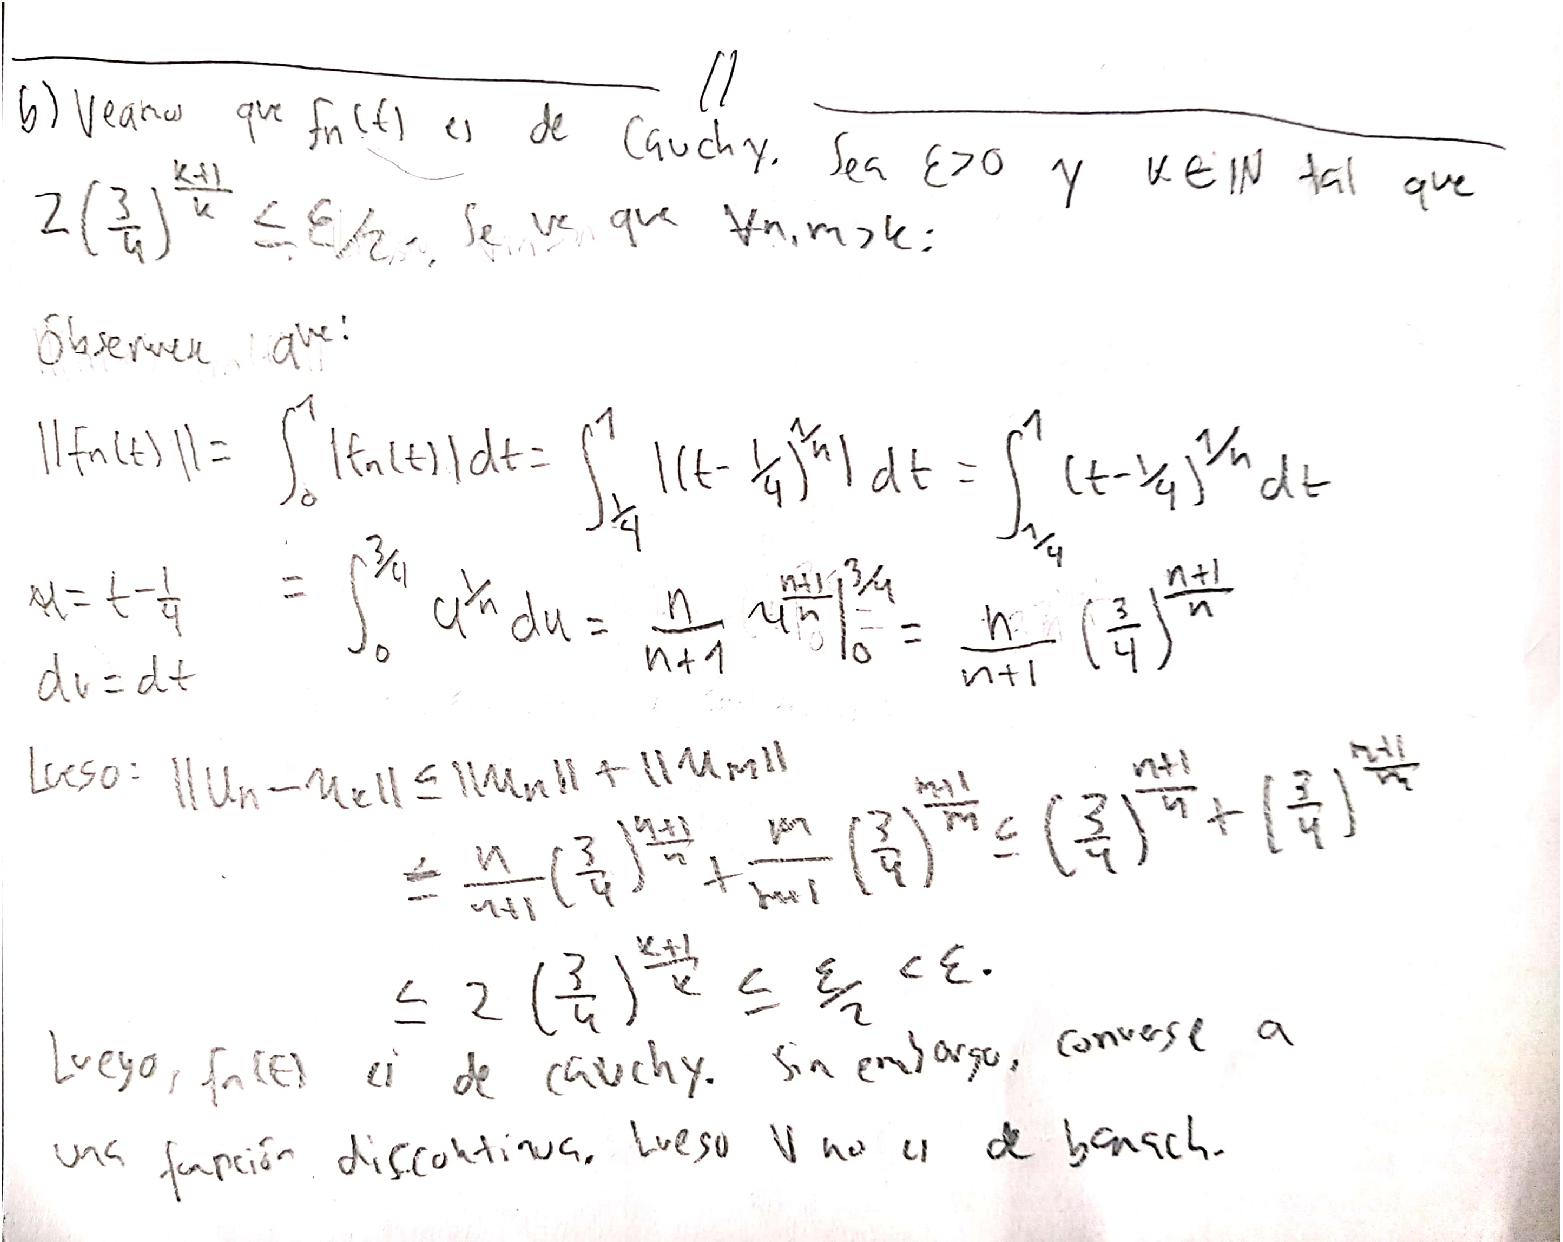
\includegraphics[scale=.6]{figs/1b}
         \end{figure}
         \newpage
         \item Item 3.
         \begin{figure}[H]
           \centering
           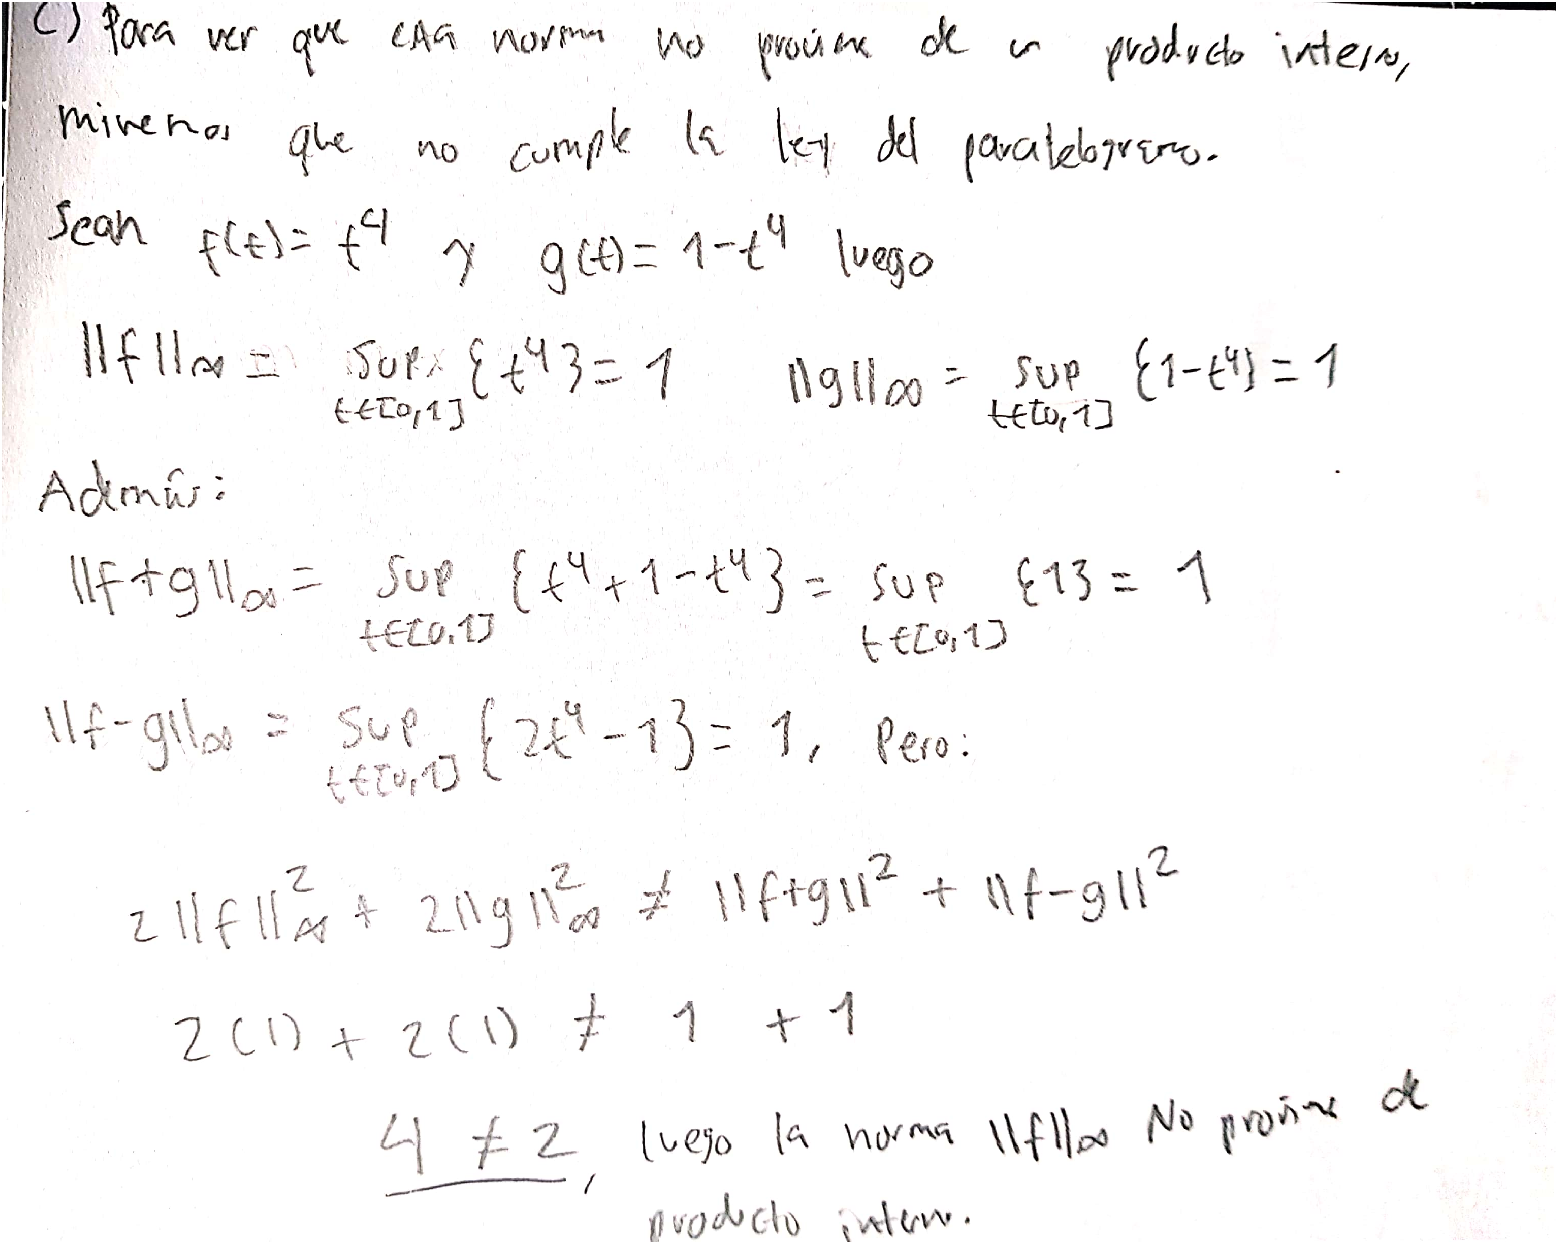
\includegraphics[scale=.5]{figs/1c}
         \end{figure}
       \end{enumerate}

     \item Pregunta 2.
       \begin{enumerate}
         \item Item 1.
           \begin{figure}[H]
             \centering 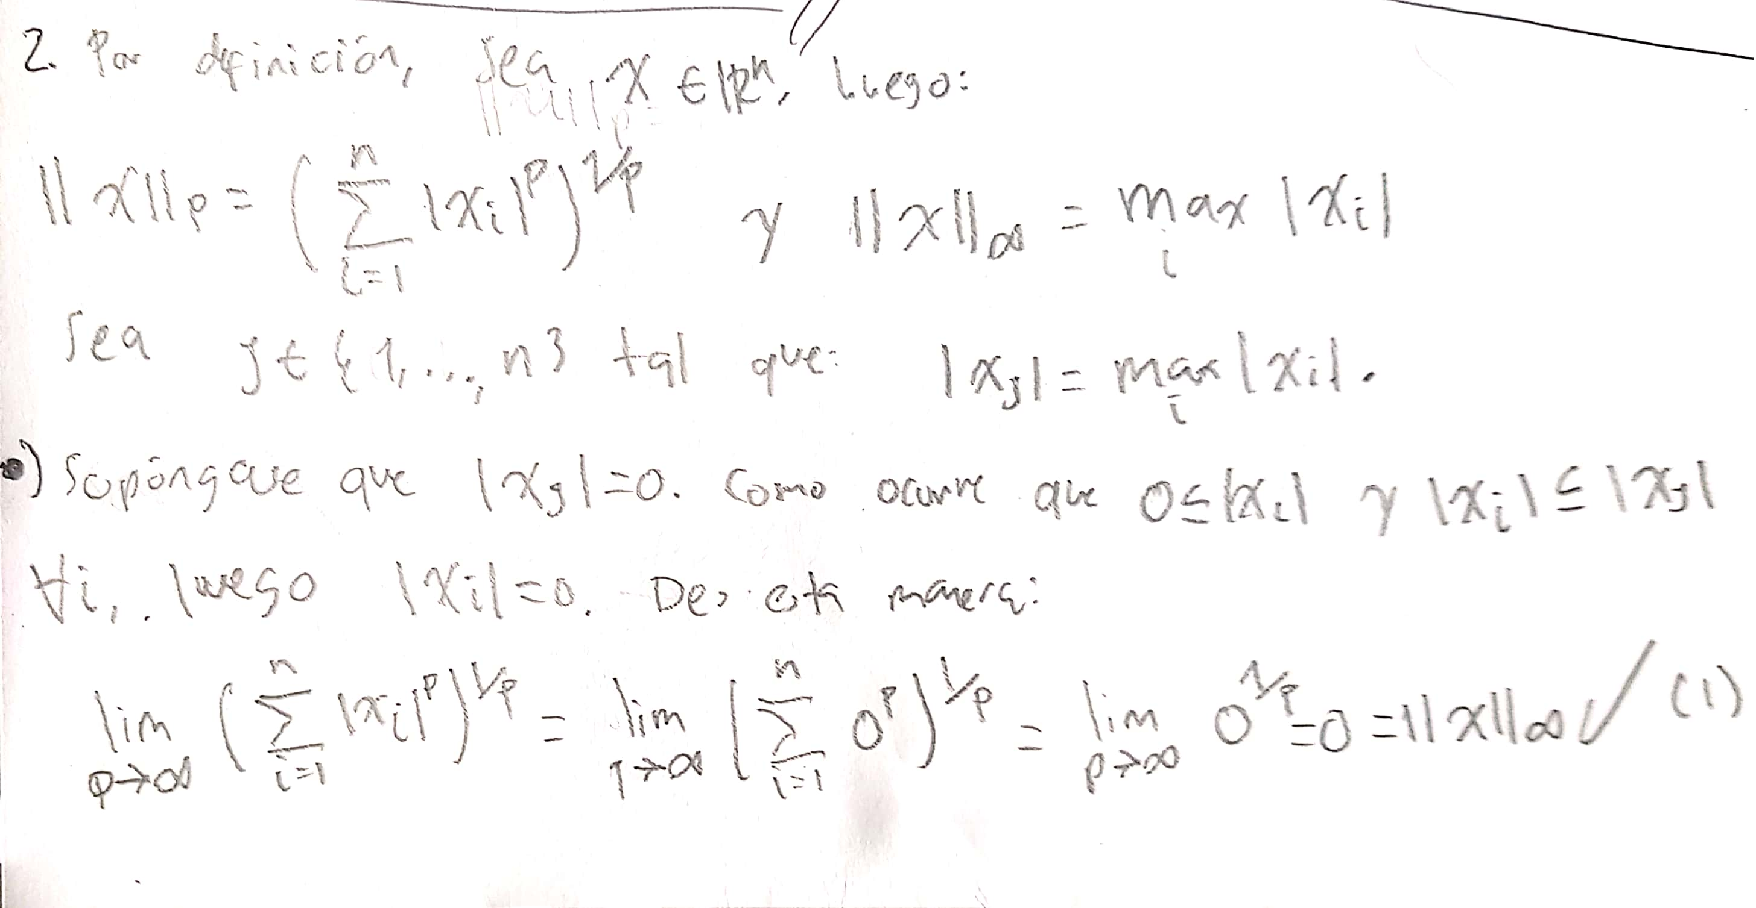
\includegraphics[scale=.5]{figs/2a1}
           \end{figure}
           \begin{figure}[H]
             \centering 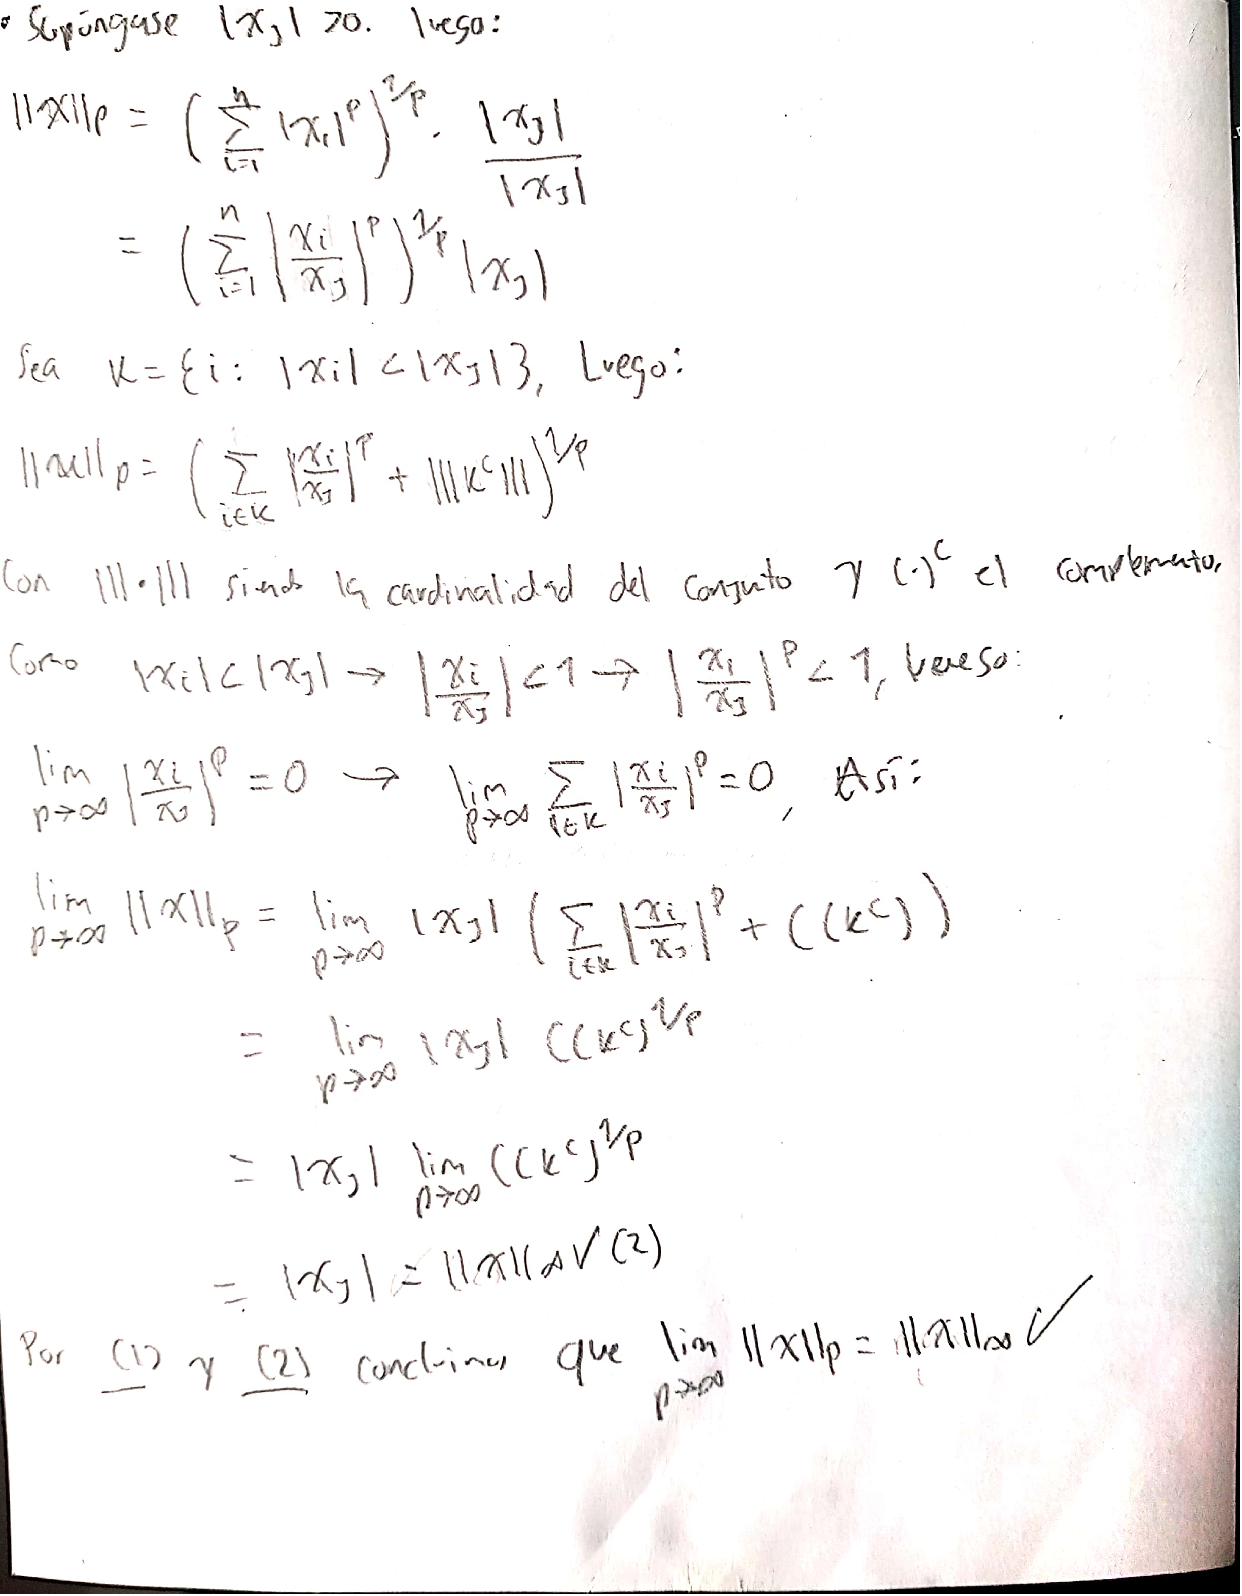
\includegraphics[scale=.8]{figs/2a2}
           \end{figure}
           \newpage
         \item Item 2.
           \begin{figure}[H]
             \centering 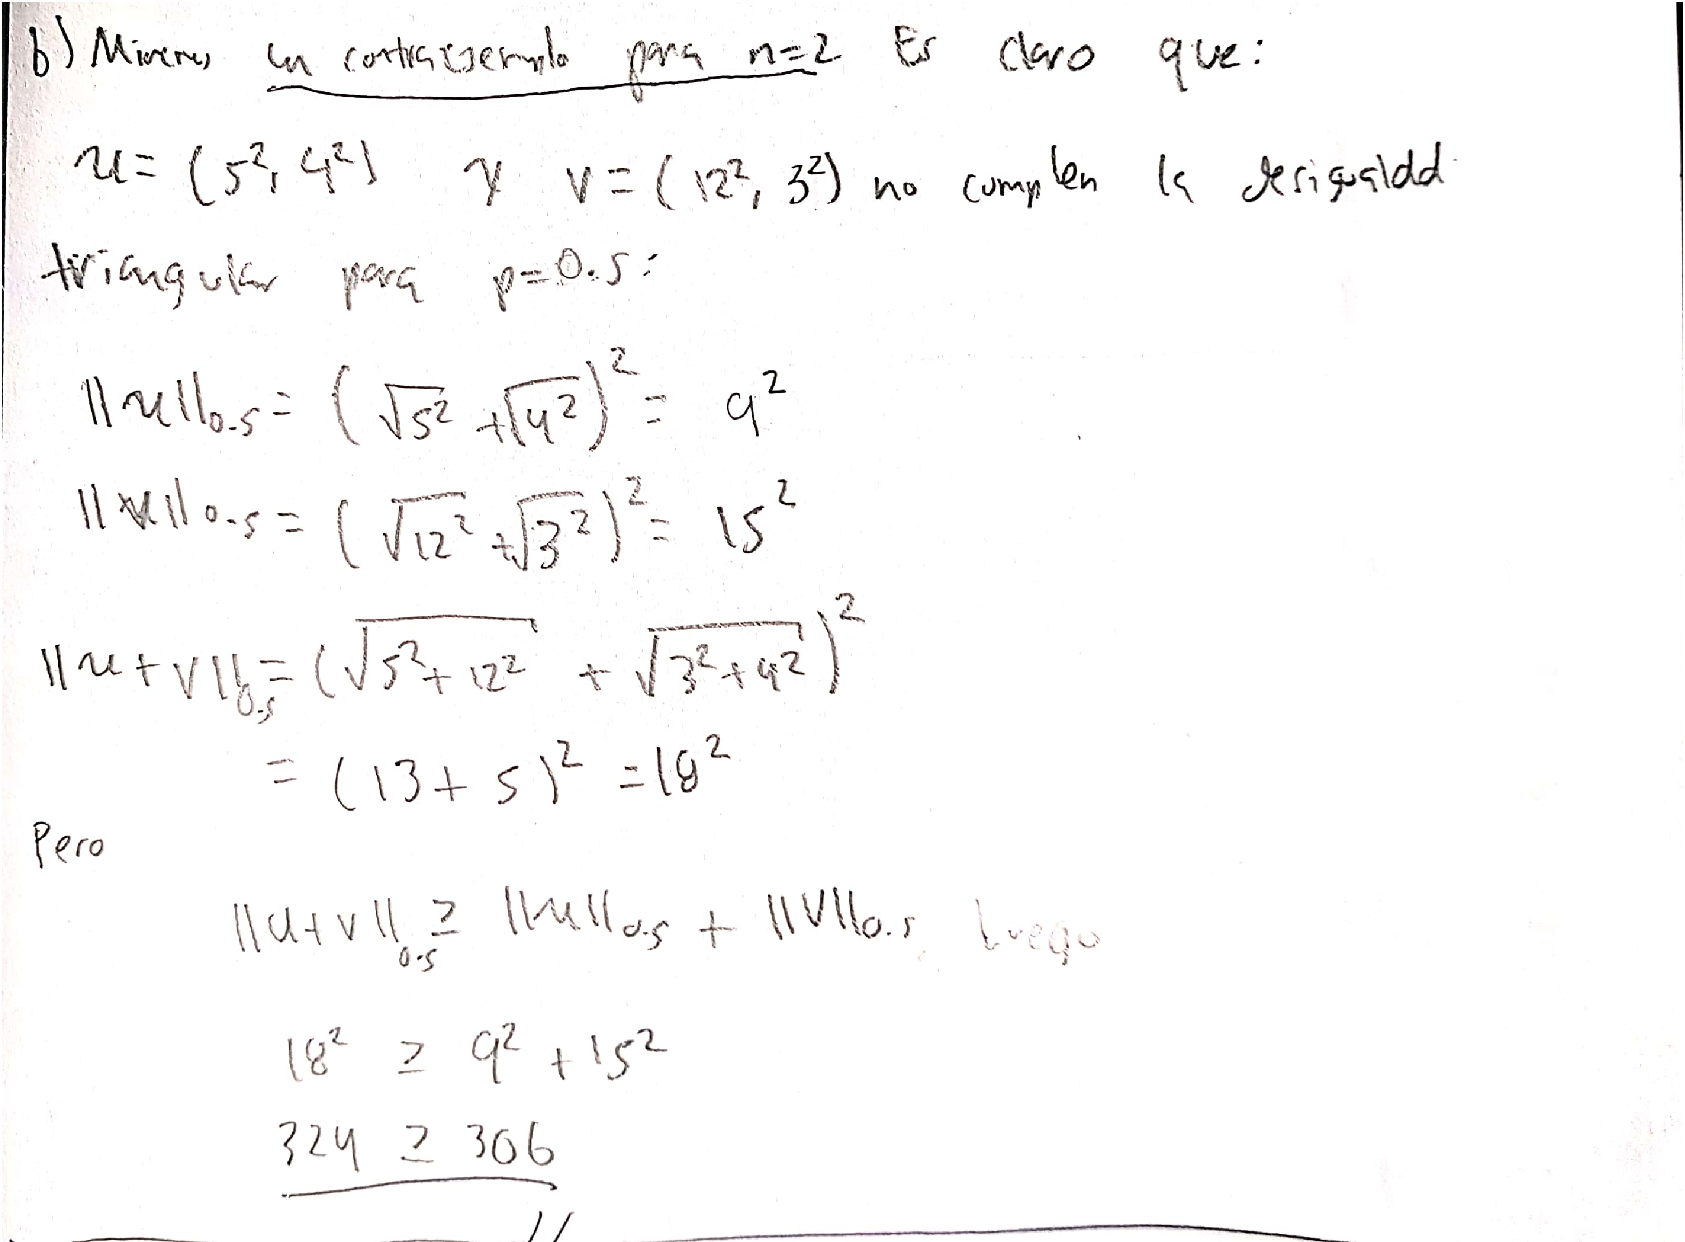
\includegraphics[scale=.5]{figs/2b}
           \end{figure}
         \item Item 3.
           \begin{figure}[H]
             \centering 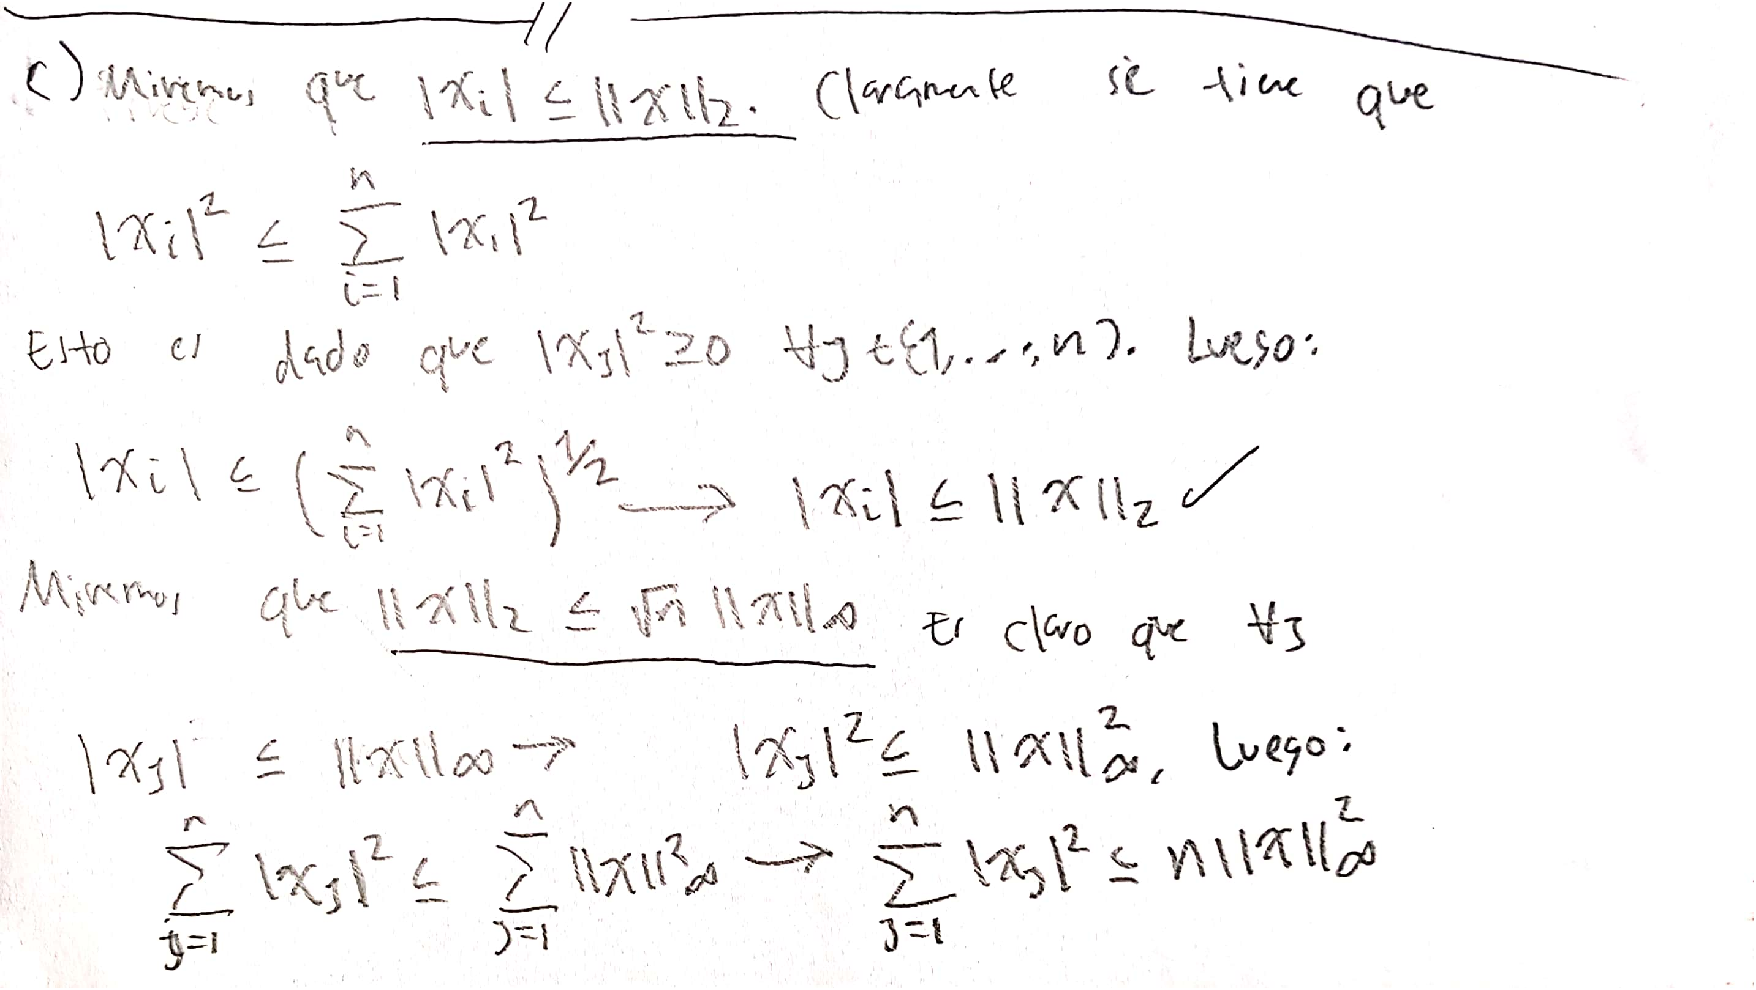
\includegraphics[scale=.5]{figs/2c1}
         \end{figure}
           \begin{figure}[H]
             \centering 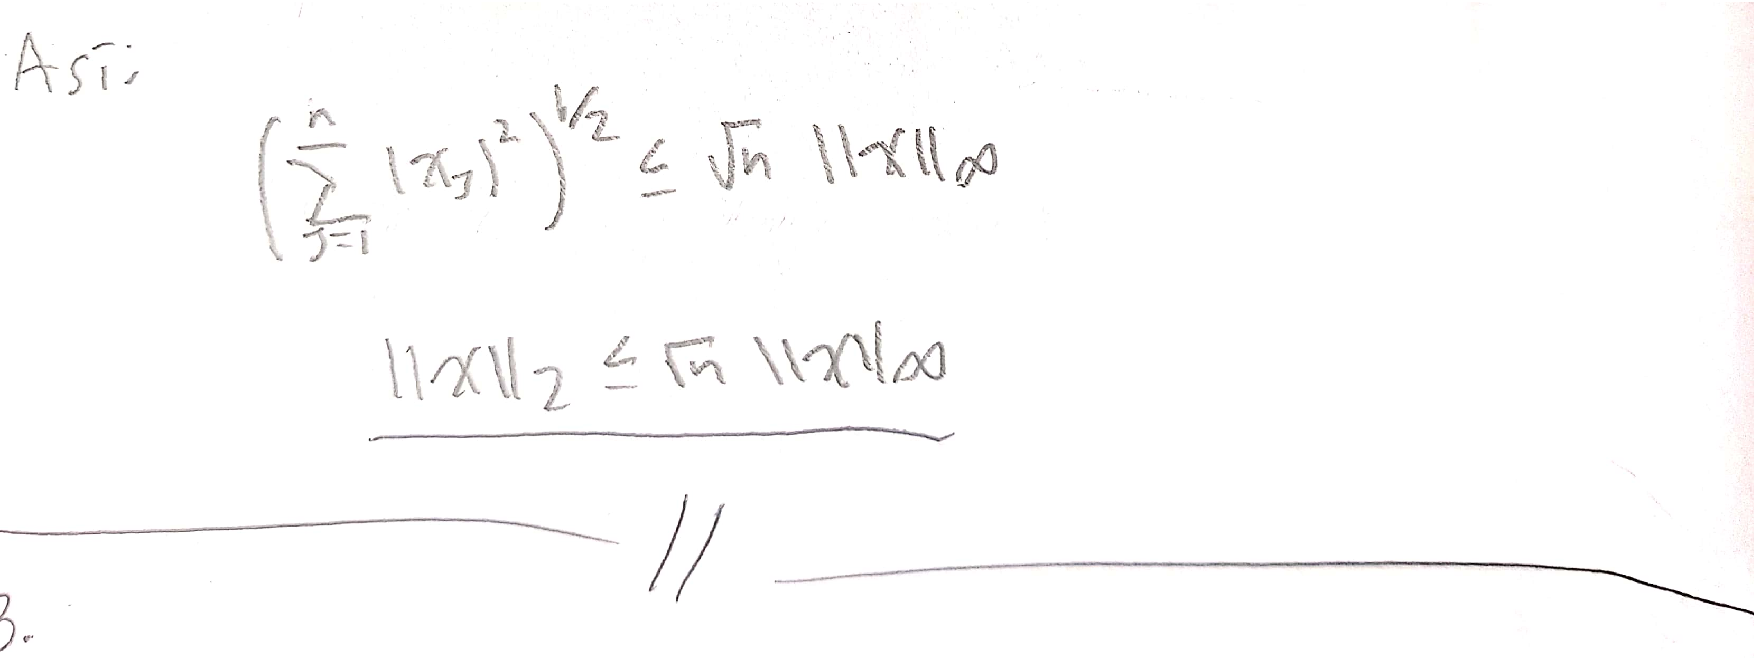
\includegraphics[scale=.4]{figs/2c2}
         \end{figure}
       \end{enumerate}

     \item Pregunta 3.
       \begin{enumerate}
         \item Item 1.
           \begin{figure}[H]
             \centering 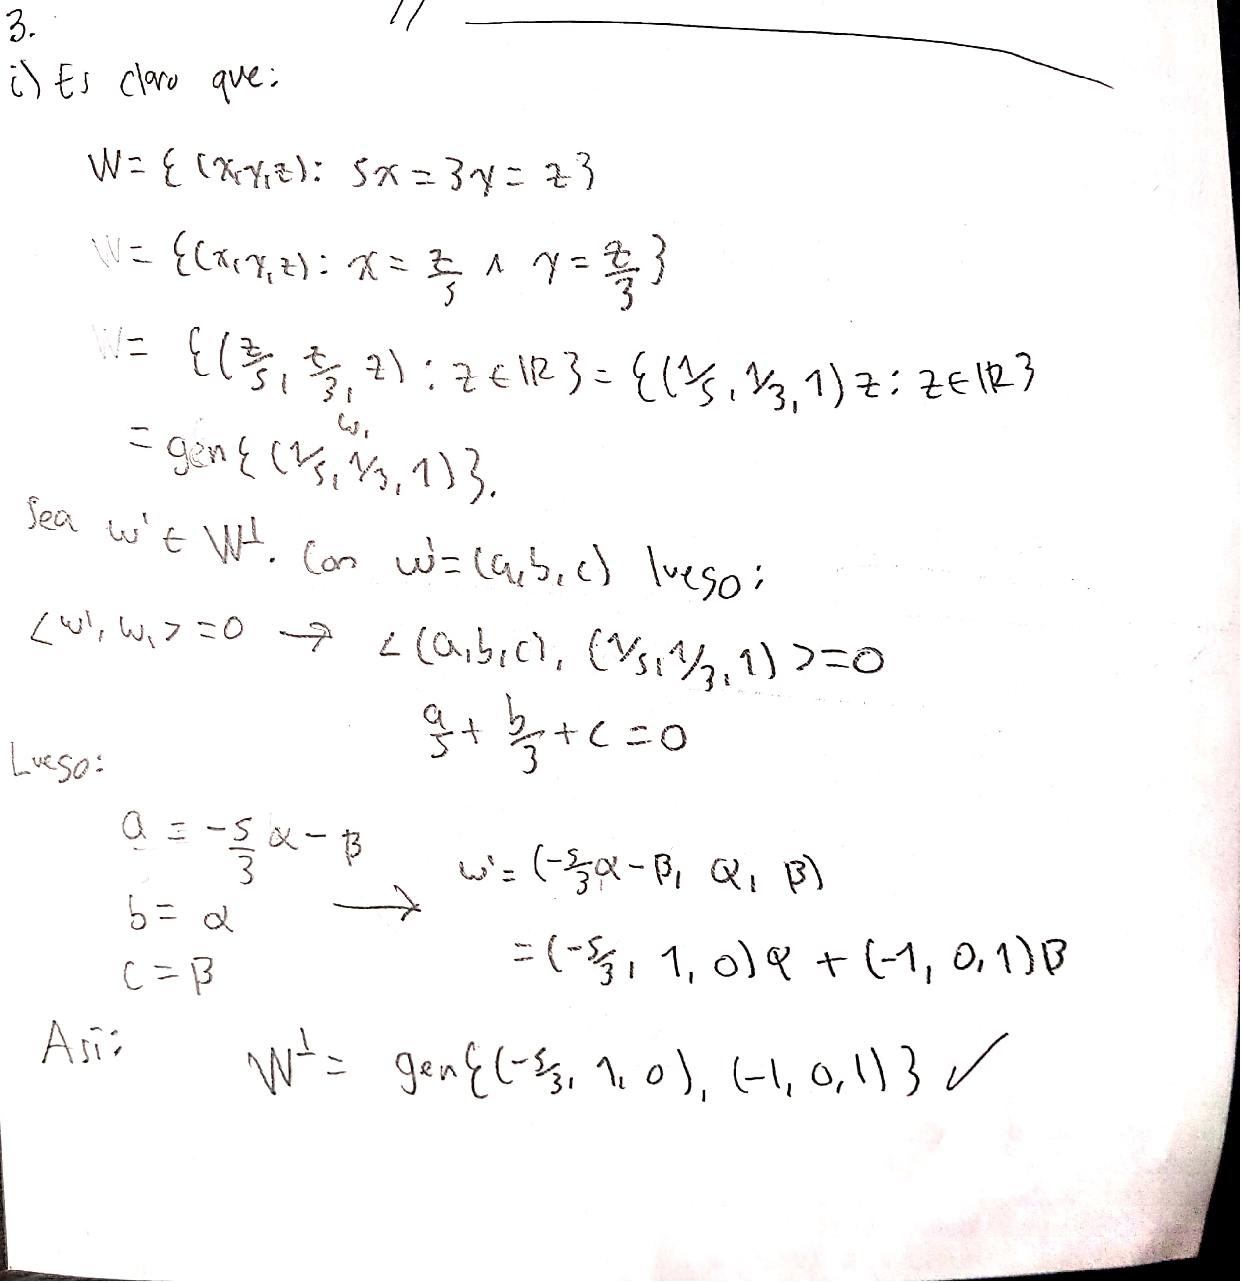
\includegraphics[scale=.55]{figs/3a}
         \end{figure} \newpage
         \item Item 2.
           \begin{figure}[H]
             \centering 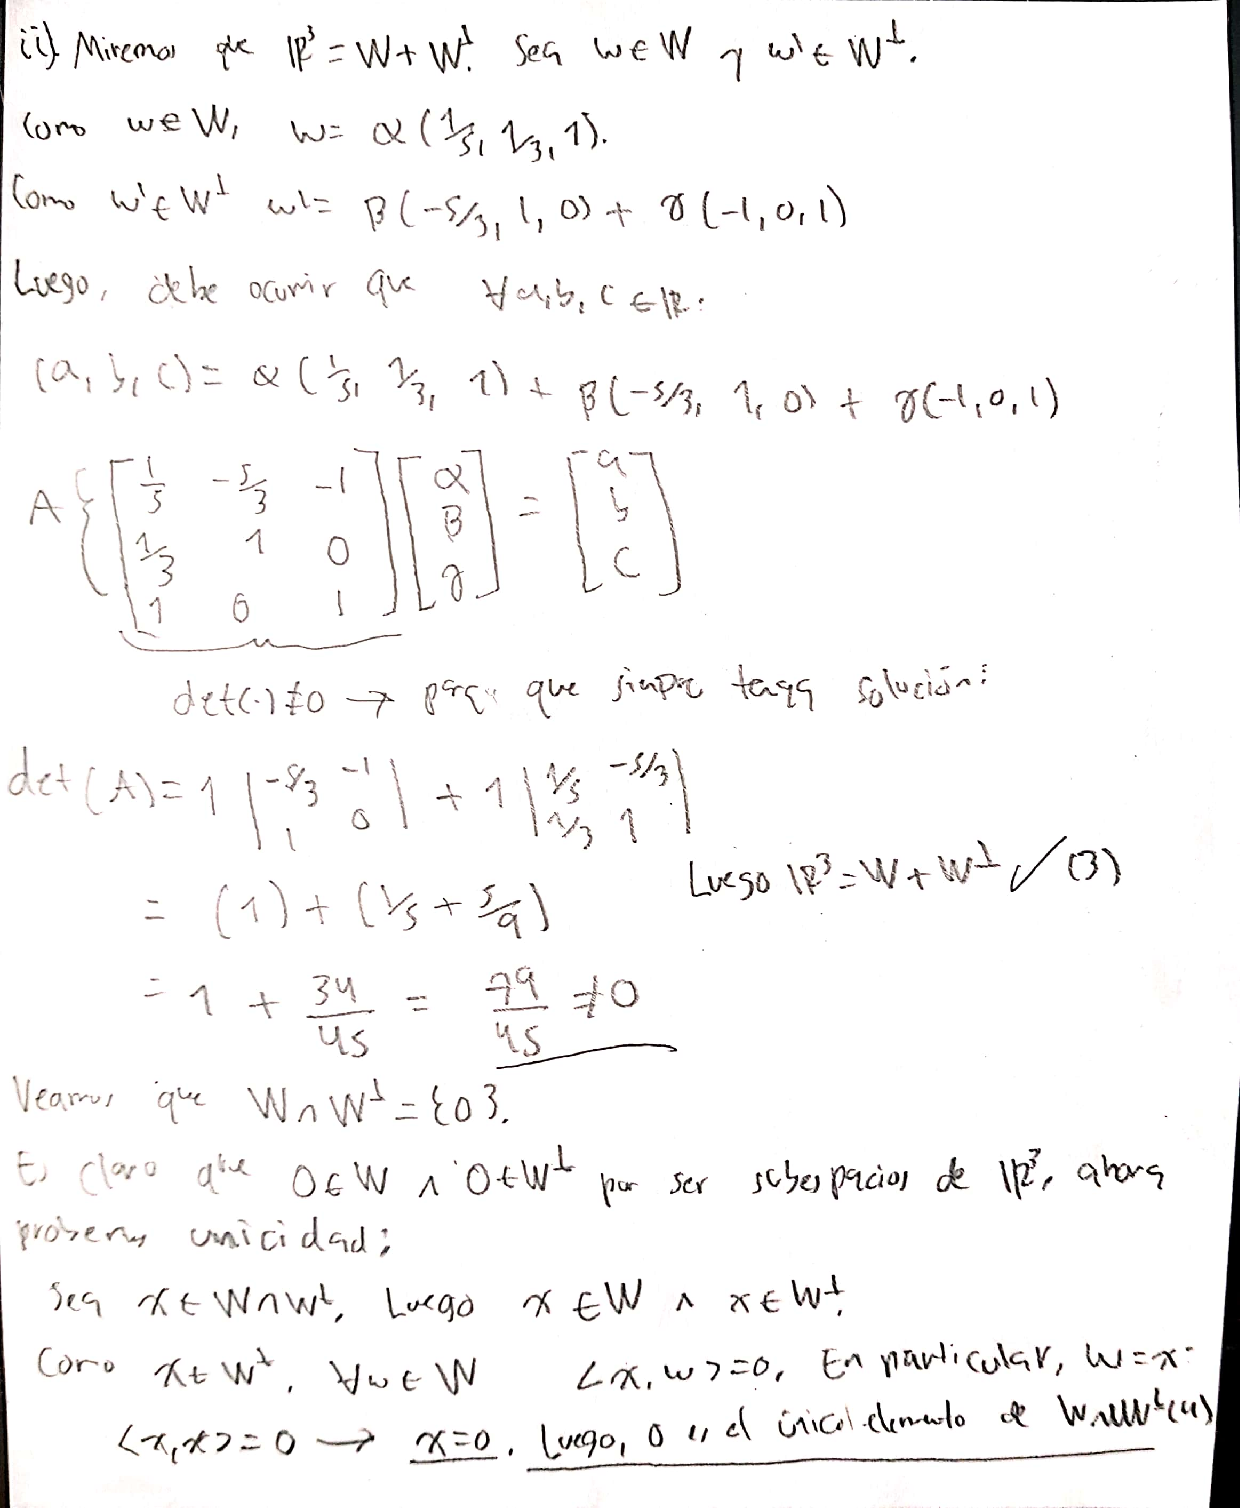
\includegraphics[scale=.6]{figs/3b1}
         \end{figure}
           \begin{figure}[H]
             \centering 
\includegraphics[scale=.4]{figs/3b2}
         \end{figure}
         \item Item 3.
           \begin{figure}[H]
             \centering 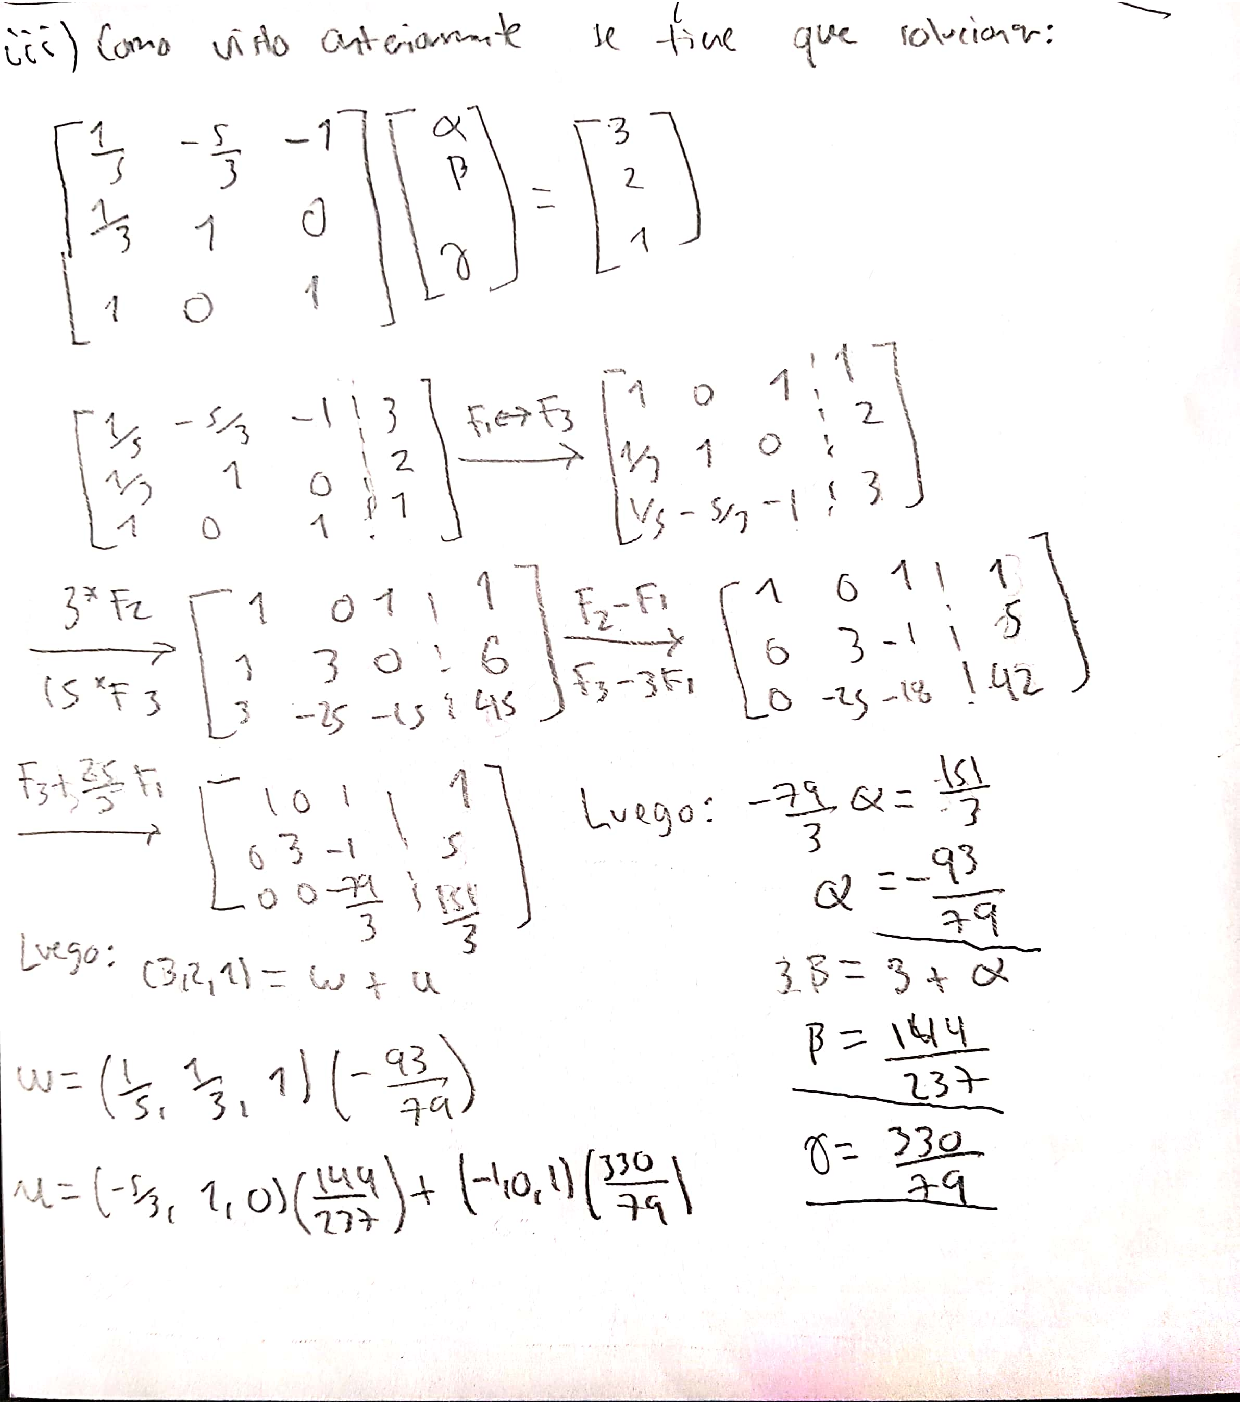
\includegraphics[scale=.8]{figs/3c}
         \end{figure}
       \end{enumerate}
   \end{enumerate}
\end{document}
